%% LyX 2.0.4 created this file.  For more info, see http://www.lyx.org/.
%% Do not edit unless you really know what you are doing.
\documentclass[oneside,dutch]{amsart}
\usepackage[T1]{fontenc}
\usepackage[latin9]{inputenc}
\usepackage[a4paper]{geometry}
\geometry{verbose,tmargin=3cm,bmargin=3cm,lmargin=2cm,rmargin=2cm}
\setlength{\parskip}{\smallskipamount}
\setlength{\parindent}{0pt}
\usepackage{float}
\usepackage{amsthm}
\usepackage{graphicx}
\graphicspath{{Figures/}}

\makeatletter
%%%%%%%%%%%%%%%%%%%%%%%%%%%%%% Textclass specific LaTeX commands.
\numberwithin{equation}{section}
\numberwithin{figure}{section}

\makeatother

\usepackage{babel}
\begin{document}

\title{Lenzen slijpen}


\author{N.G. Schultheiss}

\maketitle

\section{Inleiding}

Deze module volgt op de module ``Lenzen'' of ``Parabolische spiegels
maken''. Deze module wordt vervolgd met de module ``Telescopen''.
Uiteindelijk kun je met de opgedane kennis een telescoop bouwen en
de werking verklaren. Deze module is als een technische module op
te vatten. We onderzoeken de technieken om lenzen te slijpen.

Je kent de stelling van Pythagoras.


\section{Bollen maken}

Een bol is een figuur waarbij ieder punt van het oppervlak even ver
van het middelpunt is. Deze afstand wordt de straal genoemd. Met de
stelling van Pythagoras kunnen we een wiskundige formule voor een
bolvormig oppervlak met straal $r$ maken:

\[
x^{2}+y^{2}+z^{2}=r^{2}
\]


We kunnen kijken wat er gebeurt als we een plakje van de bol afsnijden.
We nemen bijvoorbeeld een bol met een straal van 5,0{[}cm{]} en snijden
een plakje van 1,0cm dik af. We moeten dan bij bijvoorbeeld $z=4,0[\mathrm{cm}]$
zagen:

\[
x^{2}+y^{2}+4,0^{2}=5,0^{2}\Rightarrow
\]


\[
x^{2}+y^{2}=3,0^{2}
\]


Zoals uit de formule blijkt heeft de zaagsnede een cirkelvormige vorm
met een straal van 3,0{[}cm{]}. Als we een bol hebben is dit natuurlijk
een makkelijke manier om een planconcave lens te maken. We moeten
echter eerst een bol(deel) maken.

Lenzen kunnen we slijpen als we een plaat om een as draaien en een
draaiende cilinder om een iets schuin geplaatste as laten draaien.
Als de cilinder stukjes van de plaat wegsnijdt (verspaant) krijgen
we een bol. Als eerste cilinder kun je bijvoorbeeld in een doehetzelf
winkel een rondegatenzaag kopen.

\begin{figure}[H]
\noindent \begin{centering}
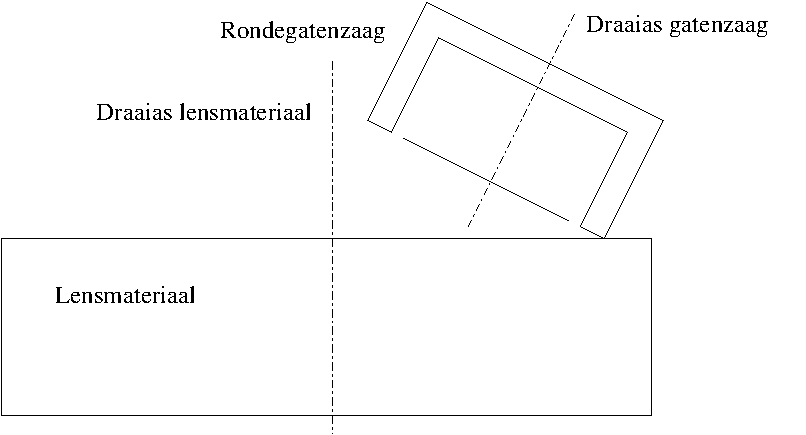
\includegraphics[scale=0.75]{slijpopstelling}
\par\end{centering}

\caption{Een opstelling om lenzen te slijpen}
\end{figure}


Het is belangrijk om de assen zo in te stellen dat de rondegatenzaag
aan de draaias van het lensmateriaal (bijvoorbeeld plexiglas) raakt.
Als alles netjes rond draait, wordt de bovenkant een bol (zonder dat
er een raar puntje overblijft). Omdat de rondegatenzaag vrij grof
zaagt, krijgen we geen mooi doorzichtig oppervlak. We kunnen de zaagbewerking
door een schuurbewerking laten volgen. Neem daarvoor een buis met
dezelfde diameter als die van de ronde gatenzaag. Op het uiteinde
van de buis doen we bijvoorbeeld schuurpapier. Een tweede methode
is om een slijppasta van water en fijn zand op het oppervlak te doen.
Daarna maken we alles schoon en herhalen het met een fijnere slijppasta
(een schoonmaakmiddel dat ``niet krast''). Tot slot gebruiken we
koperpoets. Als alles goed gaat hebben we dan een optisch zuiver oppervlak.
Als de achterkant vlak en optisch zuiver blijft hebben we een planconvexe
lens. Met de lenzenformule kunnen we uitrekenen hoe sterk de lens
wordt.
\end{document}
